\documentclass{article}
\usepackage{apacite}
\usepackage{pdfpages}
\usepackage{graphicx}
\usepackage{fancyhdr}

\pagestyle{fancy}
\fancyhf{}
\rhead{Damian Bachasingh}	
\lhead{An app being a solution for the obsolete reports}
\rfoot{Page \thepage}
\lfoot{\LaTeX}

\renewcommand{\familydefault}{pbk}		 % Bookman serif font

% dit hieronder kan alleen gebruikt worden met xetex of luatex
%\usepackage{fontspec}
%\setmainfont{Butler}

\begin{document}
\author{Damian Bachasingh}
\title{An app being a solution for the obsolete reports}
\clearpage
\maketitle
\thispagestyle{empty}

\begin{verbatim}
Damian Bachasingh	
0917993
0917993@hr.nl
Computer science at Rotterdam University of Applied Sciences 
31 March 2017
Aninka and Renee
TINBSK0113
\end{verbatim}

	\newpage
	\tableofcontents
	\newpage

\section{The problems with the current reports in elderly care}
In the elderly care the amount of elderly people increases every year. The cause of the rise in the amount is due to the baby boom generation becoming older. Their life expectancy also increases \cite{1}. The amount of nurses on the other hand decreases.
In the elderly care there are quite some problems nurses have to deal with. Things like a bad internet network and hard physical work. There is a big problem in the care that happens often and is crucial to time, being the fact that a lot of time is being taken into reporting of elderly people. 
The reporting is crucial in the elderly care, because it keeps track of a client’s progress. With this it possible to discovers problems with the client and see how and why something possibly happened \cite{2}. Reporting causes a lot of overtime, thus causing nurses to have less time left for the clients \cite{3}. This causes a bigger workload. Although they do want to spend more time it is not always  possible.        A possible solution to this is to create an automated system in which the nurses can do the administration on a smartphone.


\section{A solution}
The app is supposed to be on the smartphone. Out of 80 percent of people aged between 18 and 80  use a smartphone \cite{4}. First off is the app’s prototype meant to be developed on android. Beyond that more platforms will follow. To fully use the app, the user needs credentials to login. Only with the correct privilege, it is possible to login. More than that it is only possible to login when the user is connected to the network of the building. When logged into the app, the user is able to see information about clients they take care of. This information is private, so the app restricts screenshots. 
The App uses a grading system. For certain topics, a grade can be given ranging from 0 to 10. These topics can be health, behaviour and eating behaviour. The nurses are still required to complement additional information. But here’s is the deal. Instead of typing, the user can speak to the phone which then will be converted to text. This reduces a lot of time. Of course the text won’t always be very accurate. So the user has to occasionally correct the text with the integrated keyboard. The administrator of the app can set a minimum and maximum amount of words to maximize documentation results. The app also checks on subjectivity. It hints the user to not use words like: “somewhat”, “a bit”, “angry”, “much”. This helps the user to keep the report more objective. The app’s additional function is to create graphs from the grading system. This way it is easier to determine the clients progress. There is an app that also provides a detailed patient care report that can be completed using a Smartphone or tablet called “EMS Patient Care Report”. This app however does not make us of speech to text and smart functions
The App is time efficient, easy to use and keeps track of all things. It makes the workload a lot lighter for nurses and the patients receive more care (see figure 1). 


\subsection{Cons}
There are some cons though. This app does need some investing. The prototype will be developed on the android platform. So not all users can use the app in its prototype stage. In the Netherlands more than 50 percent of people ranging between 18 and 80 use android \cite{4}. So the amount of test users is sufficient enough.

\begin{figure}
\centering
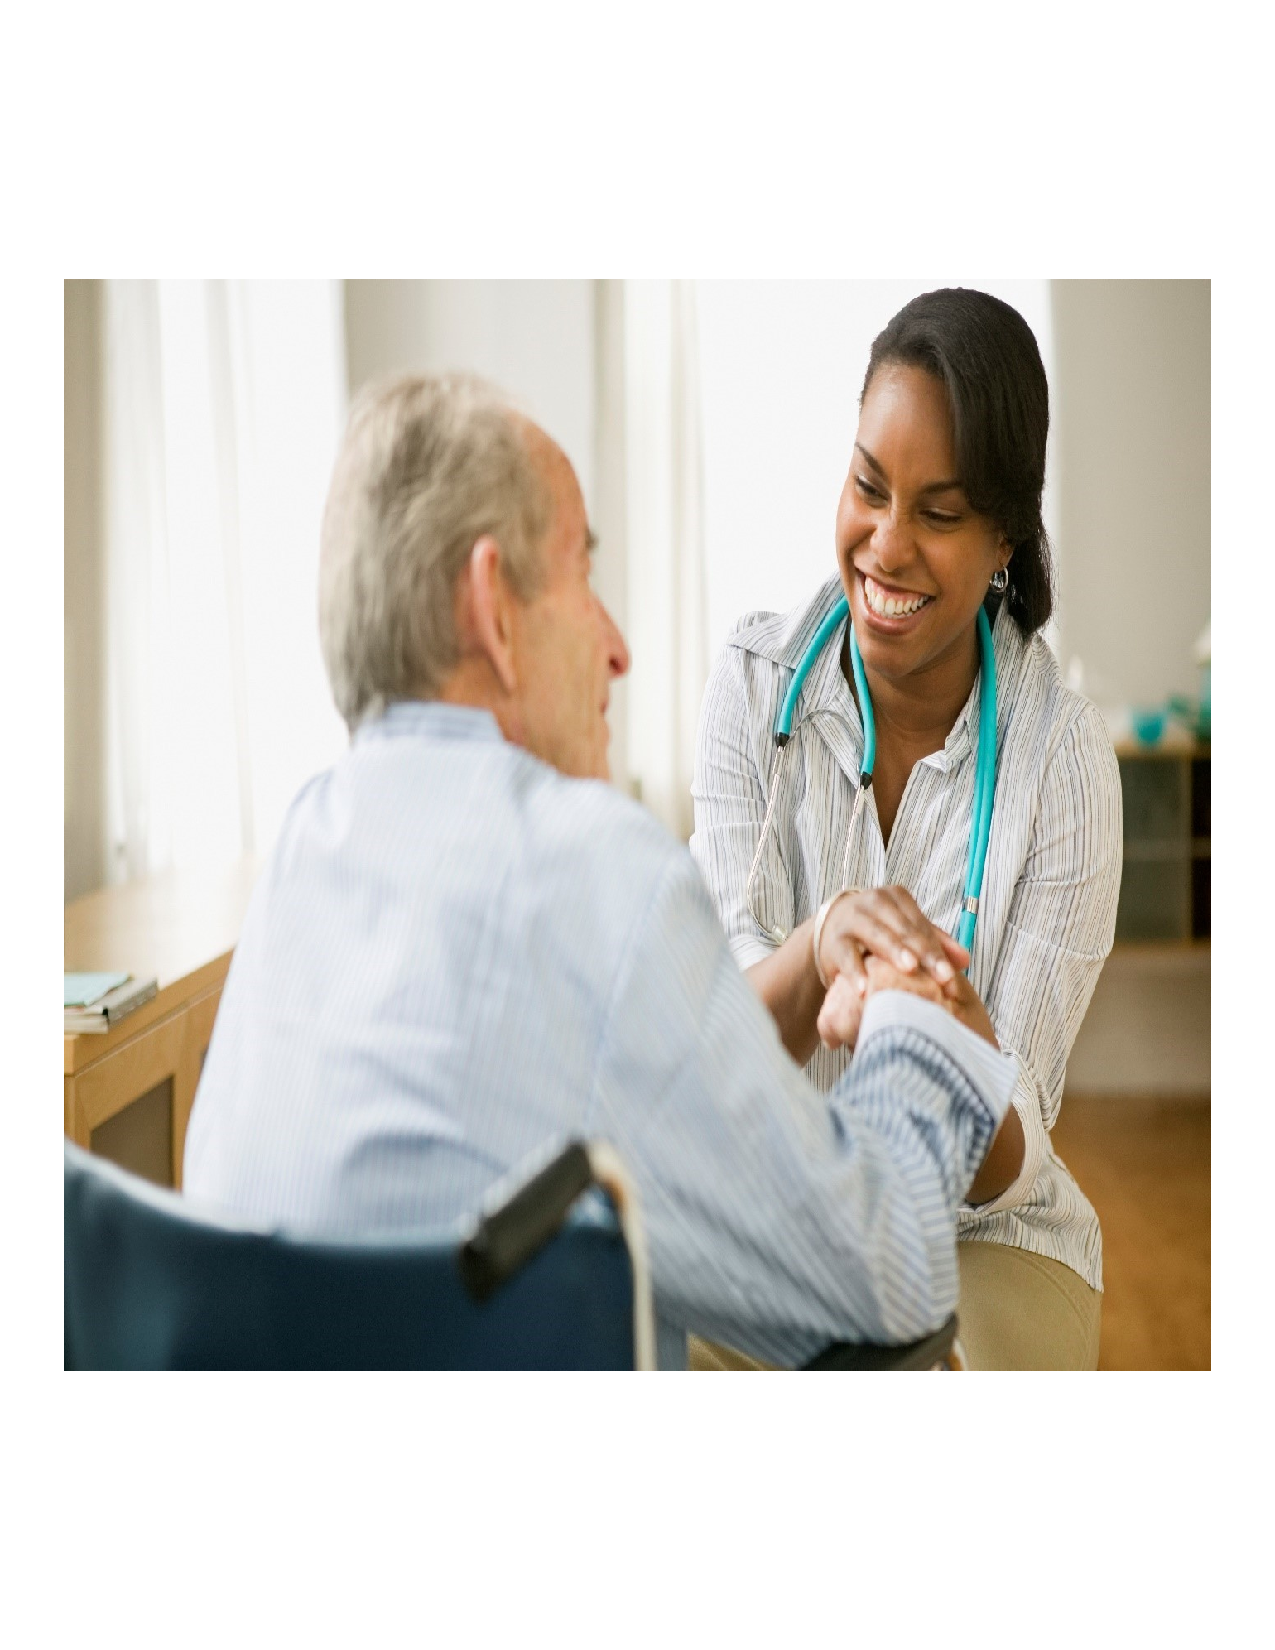
\includegraphics[width = 50mm]{care.pdf}
\caption{Care Example}
\label{fig:Care Example}
\end{figure}

\section{Results}
We wanted to find out which type of input saves the most time. We look at the types: typing on the smartphones touchscreen and speech to text. The accepted average typing speed is 41 WPM (words per minute) \cite{5}. The pace of audiobooks are around 150–160 words per minute, which is the range that people comfortably hear and vocalize words \cite{6}. Eventually this means speech to text is more than 3.5 more times efficient than typing although the speeds may vary between nurses.

\section {Conclusion}
Concluding, the reporting currently takes too much time and is not filtered and yet reports are crucial in the elderly care. There is a solution as described as above, we have developed an app, that does reduce the workload on nurses and creates more time for the clients. The app is ethically and security wise in good state.

	\newpage
\bibliographystyle{apacite}
\bibliography{verwijzingen}
\end{document}
